\section{Position Specific Scoring}
\subsection*{Implementieren Sie in einer Programmiersprache Ihrer Wahl ein Framework für positionsspezifisches Scoring.}

% Diese Aufgabe wurde in Google Programmiersprache Go umgesetzt, da diese neben intuitiverer Syntax als
% andere Programmiersprachen auf Typsicherheit setzt. Das git repository für
% die Aufgabe findet sich unter github.com/rathalos64/algo5.

% Der geschätzte Arbeitsaufwand beträgt ~12h.

% \bigskip\noindent
% Die Struktur der Abgabe besteht aus den folgenden Files.
% \newline
% \dirtree{%
% 	.1 /root .
% 	.2 main.go .
% 	.2 hmm.go .
% 	.2 sequence.go .
% 	.2 forward.go .
% 	.2 structs.go .
% 	.2 utils.go .
% }

% \bigskip
% Kurz zur Erklärung der einzelnen Files.
% \begin{itemize}
% 	\item \textbf{main.go} präsentiert das Hauptprogramm, welches die Models und Sequenzen einliest, validiert und
% 	anschließend evaluiert.
% 	\item \textbf{hmm.go} definiert die Struktur eines Hidden Markov Models mitsamt Contraints und Mappingnamen für 
% 	Se-/Deserialisierung.
% 	\item \textbf{sequence.go} definiert die Struktur einer Sequenz von Beobachtungen mitsamt Contraints und Mappingnamen für 
% 	Se-/Deserialisierung.
% 	\item \textbf{forward.go} implementiert den Forward-Algorithmus über die Funktion \textit{Evaluate()}.
% 	\item \textbf{structs.go} definiert Hilfstypen (u.a für die Validierung).
% 	\item \textbf{utils.go} definiert Hilfsfunktionen
% \end{itemize}

% \noindent
% Das Programm arbeitet mit Inputfiles, welche zum Definieren von HMMs und Sequenzen verwendet werden.
% Als Fileformat wird JSON verwendet aufgrund Go's nativer Se-/Deserializierungstechnik. Zudem sind JSON files 
% leichter lesbar und in vielen Webanwendungen standardisiert in Verwendung. Das Programm verwendet genau ein JSON file für
% das Einlesen von verschiedenen Modellen [Listing 1] und eines für das Einlesen der Beobachtungssequenzen [Listing 2].

% \pagebreak
% \newgeometry{top=3.04cm, bottom=3.54cm, left=2.04cm, right=2.04cm}
% \lstset{
% 	string=[s]{"}{"},
%     stringstyle=\color{Blue},
%     comment=[l]{:},
% 	commentstyle=\color{Black},
% 	numbers=none
% }
% \lstinputlisting[caption={models.json. Zu sehen sind hier drei Modelle, welches das Wetter simulieren sollen. 
% Zu beachten sind die jeweils leichten Veränderung in PI, A und B. Durch diese Parameterveränderung, wollen wir später sehen, welches
% der Modelle am Wahrscheinlichsten Beobachtungssequenzen erzeugt haben könnten.}, captionpos=b]{../examples/models/models.json}

% \lstinputlisting[caption={sequences.json. Hier zu sehen sind drei Definitionen für Beobachtungssequenzen. Die eigentliche Beobachtungssequenz
% wird über das Feld ``observations'' definiert. Das Feld ``hmm\_ids'' beinhaltet die IDs der Modelle, gegen diese getestet werden soll. Es 
% ist offensichtlich, dass die IDs von Modellen stammen müssen, welche existieren. So wird ersichtlich, dass z.b.: die Sequenz ``sequence\_01''
% gegen all Modelle getestet wird.}, captionpos=b]{../examples/sequences/sequences.json}

% \noindent
% Das Programm wurde für die Konsole entwickelt und verwendet daher Kommandozeilenparameter um die Inputdaten einzulesen [Listing 3].
% \begin{lstlisting}[language=bash, caption={Beispielaufruf am Terminal}, captionpos=b]
% $ ./hmm -models examples/models/models.json -sequences examples/sequences/sequences.json
% \end{lstlisting}

% \noindent
% Hat das Programm erfolgreich die Inputfiles eingelesen und deren Korrektheit validiert, printet
% das Programm sofort das Ergebnis auf das Terminal. Es wird zu jeder Sequenz alle Wahrscheinlichkeiten (Likelihood \& Loglikelihood) 
% der jeweiligen Modelle sowie das wahrscheinlichste (likeliest) Modell ausgegeben [Abbildung 1].

% \pagebreak
% \begin{wrapfigure}{i}{0.5\textwidth}
% 	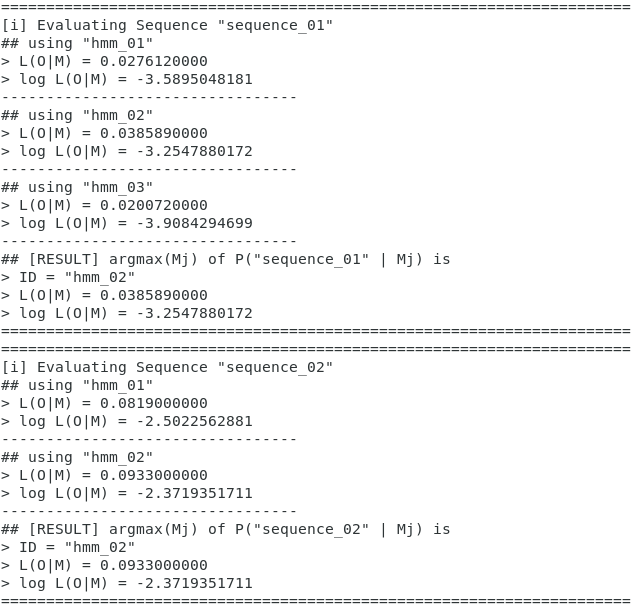
\includegraphics[scale=0.7]{../screenshots/result.png}	
% 	\centering
% 	\captionsetup{}
% 	\caption{Ein Ausschnitt des Terminals. Zu jeder Sequenz ermittelt das Programm
% 	das Modell, welches die Sequenz am Wahrscheinlichsten erzeugt haben könnte.}
% \end{wrapfigure}

% \pagebreak
% \newgeometry{top=3.04cm, bottom=3.54cm, left=2.04cm, right=2.04cm}
% \lstset{
% 	stringstyle=\color{Red}\ttfamily,
% 	commentstyle=\color{Green}\ttfamily,
% 	numbers=left
% }
\pagebreak
\lstinputlisting[language=Python, caption={main.py}]{../pss/main.py}

\pagebreak
\lstinputlisting[language=Python, caption={pss.py}]{../pss/pss.go}

\pagebreak
\lstinputlisting[language=Python, caption={pss_sequence.py}]{../pss/pss_sequence.py}

